% !TeX root = ../main.tex

\chapter{緒論}

地球作為一顆動態的行星,其內部動力學相當複雜。地球動力學(Geodynamics)由地球(Geo-)與動力(dynamics)兩個詞所組成,顧名思義為探討地球內部的動力過程,以及地球內部物質受力後所發生的變形作用。
地質學之父查理斯萊爾爵士(Sir Charles Lyell)在<<地質學原理(Principles of Geology)>>(\citealp{lyell2009})一書中提出一句話「現在是通往過去的一把鑰匙」,表示過去所發生的地質事件與現在進行中的地質作用皆相同。

人類在很早之前便知道地球有動態過程,例如地震與火山爆發。
早期的地球科學研究侷限於地表觀察,儘管在牛頓力學成為自然科學的顯學後,以物理基礎定量描述自然現象與作用力已被廣泛應用,但由於地質作用之時間尺度遠超乎當時定年技術的範疇,因此地球內部之構造活動尚無人知曉。
至19世紀,隨著人類在實驗與測量技術上的突破,藉由物理方法探測地球內部的技術才開始被應用到對地球內部的觀察,然而當時的地球物理學門與地質科學是完全分開的領域。
直到板塊構造學說被提出,地球內部的驅動力可以藉由隱沒板塊水平運動所實現,顛覆地質構造由垂直運動所主導的地槽學說概念。
至此,地球科學從定性的地質描述轉變成定量的物理展現,由板塊運動所引起的地質現象在時間與空間上有最大程度的整合,該理論被稱為地球科學上的科學革命。
從此,人類可以藉由簡單的物理力學模型描述已發生的地質事件,近一步預測未來的地質構造。

計算機模擬是在計算機上執行數學建模的過程,被用來預測物理系統與現實世界的行為與結果。
該技術可以在成本較少的狀態下實現結果的推斷,量化模型實現後的不確定性,因此,計算機模擬已經大量被運用在社會科學、醫療科學、工程學與自然科學上。
地球動力學研究中,使用電腦建立地質模型,並且利用數值方法計算模擬地球內部的演化,便是一種計算機模擬。對於相對簡單的過程,模型中的物理方程式可以使用解析解或半解析解模型(e.g., Lamb, 1879; Samuel and Bercovici, 2006; Montési and Behn, 2007),不過如果需要描述較複雜的物理機制,在既定物理假設下的數學方程組只能用數值方法進行計算(詳見第二章),此時模型稱作地球動力學的數值模擬(geodynamic processes with numerical techniques)(\citealp{101Geodynamics})。

自板塊構造學說被提出以來,實現動態地球的隱沒帶系統無論在巨觀尺度下構造的演化,界觀尺度下岩石的變形狀態或微觀尺度下礦物的排列與物質置換皆是人類致力於研究的目標。
作為板塊構造運動的主要驅動力,隱沒帶系統是主要的火山與地震活動來源,過程牽扯到多尺度地質作用事件,包含緩慢的岩石脫水相變、岩漿演化與瞬態的岩石破裂。
隱沒帶數值模擬可以利用假設的物理約束與岩石流變行為預測隱沒帶內部的演化過程(\citealp{Gerya2011}),自從第一篇二維隱沒帶數值模型文章(\citealp{minear1970thermal})發布以來,地球動力學數值模型研究已經是發展成熟且被廣泛應用的地球科學學門。

這50年來的隱沒帶數值模型研究進展很大程度上取決於電腦運算速度。
早期的研究大多利用簡單的數值設定考量獨立物理參數的影響,目的是研究獨立物理參數中與隱沒模型的關係,與自然界現象有出入。
自21世紀以來,隨著電腦運算技術進步快速,數值模型研究的技術也跟著成長。
大多數的[增加本研究數值模型與過去模型的不同:加入岩漿、加入蛇紋岩化、加入相變、加入彈性變形(可得地表高程)]

\section{背景}

板塊構造學說主張地球最外層之剛性殼體---岩石圈為地表水平運動單位。
因地球內部的熱引起重力不穩定而導致岩石圈在軟流圈上水平運動(\citealp{jordan1978composition})。
岩石圈斷裂成許多剛性塊體,該塊體被稱為板塊。
大部分由板塊水平運動所引起的變形作用發生在板塊邊界。
在聚合板塊邊界,板塊發生破壞,包含碰撞與隱沒; 在分離板塊邊界,板塊發生增生,代表構造為海底擴張;錯動邊界中板塊不會顯著發生增生與破壞,代表構造為轉型斷層。

在聚合板塊邊界,溫度較冷的板塊隱沒進入地球內部,同時因溫度差所引起的密度差導致重力不穩定區形成。
隨著隱沒板塊帶著較冷物質進入地函深處,周圍壓力逐漸上升,岩石發生相變,隱沒板塊因成分與溫度與地函物質不同,溫度上的差異造成更大的重力不穩定。
在同等深度下,海洋地殼上的玄武岩最終相變成榴輝岩(eclogite)相,其為變質岩中密度最大的岩石,約落在3600-3800 $kg m^{-3}$之間,比重遠大於周圍地函。
所有的隱沒帶P-T路徑皆會通過榴輝岩(eclogite)相區(\citealp{gerya2002exhumation}; \citealp{syracuse2010global}; \citealp{penniston2015global})(見圖\ref{fig::global_subduction_eclogite})。
玄武岩相變榴輝岩的克拉伯隆斜率(Clapeyron slope)大於零(見圖\ref{fig::global_subduction_eclogite}),該相變會在隱沒板塊上較低溫的區域發生,因此於隱沒帶剖面上的同等深度中,在相變影響與溫度影響的加持下,造成隱沒板塊有足夠大的重力不穩定成為隱沒板塊持續下沉進入地球內部更深處的驅動力。
隱沒板塊上的聚合板塊稱為上覆板塊。
隱沒板塊為板塊移動與張裂的主要驅動力(\citealp{turcotte2002geodynamics})。
作為岩石圈上最巨大的不均質構造,隱沒帶將許多地表的物質帶入地球內部,在岩石圈與軟流圈之間發生複雜的物理與化學作用。隱沒板塊上的沈積物隨著周遭環境壓力與溫度逐漸升高,發生壓密作用(compaction),同時隱沒板塊上的岩石因壓力增大而將孔隙水排出,釋放進入弧前地殼區域; 在更深處,隱沒板塊上的含水礦物發生脫水作用,這些流體被釋放進入地函中,部分流體導致蛇紋岩化橄欖岩(serpentinitzed peridotite)生成,另外部分流體降低地函橄欖岩熔點,在上覆板塊側發生岩漿作用。隱沒帶中所產生的各種作用皆會對隱沒板塊動力學造成影響,因此,自然界中上部地函以上之隱沒幾何剖面有相當大的相異性,有許多原因影響隱沒傾角與隱沒曲率(\citealp{schellart2020control})。

\begin{figure*}[ht!]
    \centering
    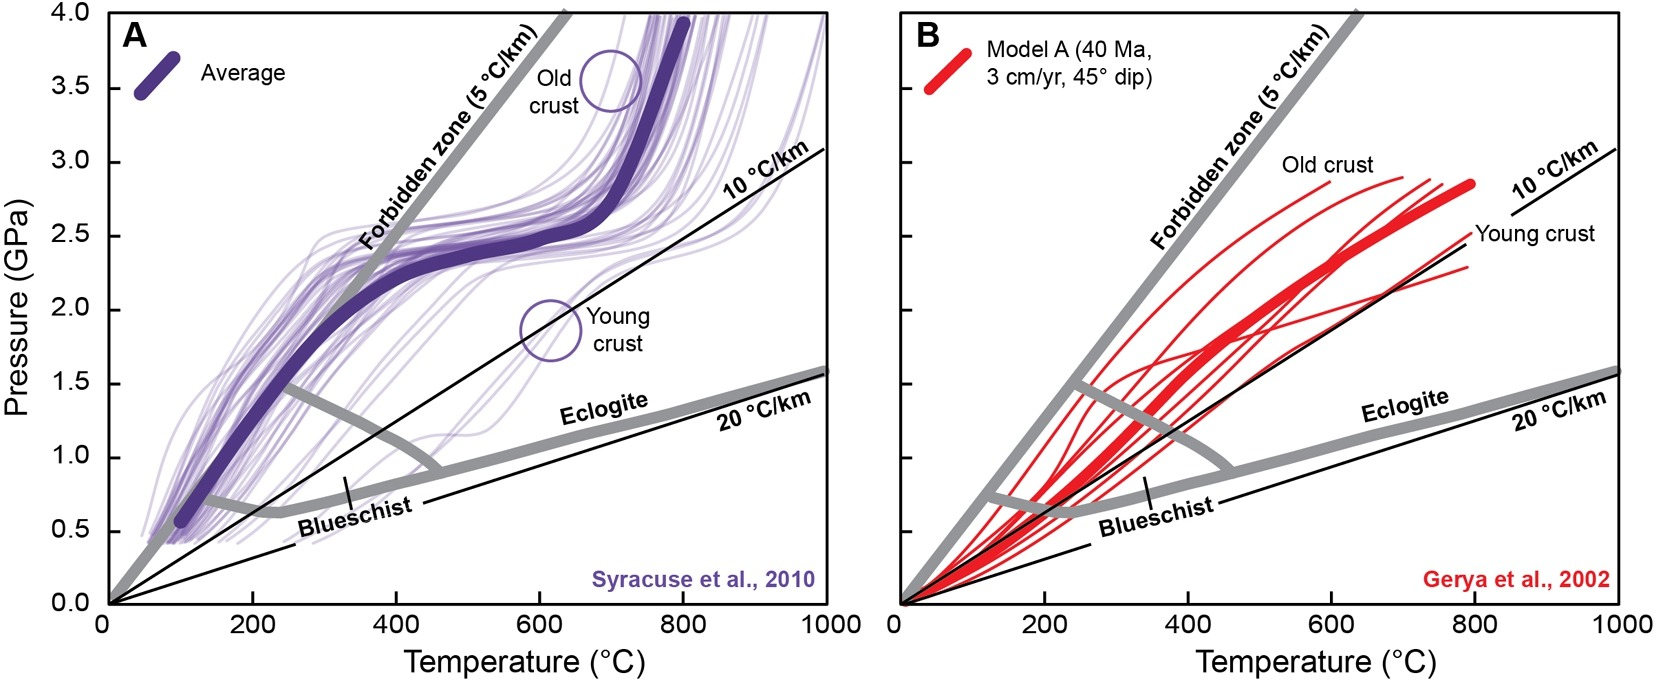
\includegraphics[width=6in]{global_subduction_eclogite.jpeg}
    \caption{
    全球隱沒板塊頂部的預測P-T路徑圖,摘自\citealp{penniston2015global}。圖中標示每公里5$^\circ$、10$^\circ$、20$^\circ$的地溫梯度與藍閃岩、榴輝岩溫壓位置。(A)來自\citealp{syracuse2010global}的全球隱沒板塊P-T路徑圖(紫色線)。(B)來自\citealp{gerya2002exhumation}的模型,紅色線代表不同年齡的隱沒板塊P-T路徑圖。
    }
    \label{fig::global_subduction_eclogite}
\end{figure*}


平坦隱沒(Flat slab subduction)是一種特殊的隱沒帶,有別於一般的隱沒板塊由於重力不穩定而下沈進入地函,平坦隱沒系統中的隱沒板塊在地函淺部(<200公里)出現一段趨近於水平的幾何構造,該水平段可長達400公里。
\citealp{barazangi1976}利用南美洲區域震源位置資料判斷秘魯與智利下方的隱沒板塊處於水平狀態,是最早發現平坦隱沒的研究。然而目前造成平坦隱沒發生的機制眾說紛紜。

從物理的角度來看,造成隱沒板塊的傾角變化可以用力矩來解釋(\citealp{stevenson1977angle}),見圖\ref{fig::Torque}。
施加於隱沒板塊上的兩個轉動力矩分別為重力力矩(gravity torque)與動水壓力矩(hydrodynamic pressure torque)(\citealp{McKenzie1969})。
重力力矩主要來自隱沒板塊與周遭地函的密度差,在圖\ref{fig::Torque}上的方向永遠是順時針。
而動水壓力矩來自隱沒板塊下地函與隱沒板塊上地函楔的壓力差,在圖\ref{fig::Torque}上的方向永遠是逆時針。

\begin{figure*}[ht!]
    \centering
    \includegraphics[width=6in]{Torque.pdf}
    \caption{隱沒系統中的施加於隱沒板塊上的轉動力矩,包含重力力矩與水壓力矩
    }
    \label{fig::Torque}
\end{figure*}

隱沒板塊的重力力矩直接與隱沒板塊有關,因此過去有不少數值模型改變隱沒板塊上的物質狀態形成平坦隱沒,例如,在隱沒板塊上放置一段增厚海洋地殼(\citealp{van2002role}; \citealp{Liu2016}; \citealp{Hu2016}等)、延後生成高密度的榴輝岩相或不生成榴輝岩相(\citealp{van2002role})、降低隱沒板塊整體密度(\citealp{Gerya2009})、設計斷掉的隱沒板塊(\citealp{Liu2016})等。
由於早期認為平坦隱沒的生成與隱沒板塊有直接關係,因此過去的數值模型研究在這方面已經相當豐富。
動水壓力矩則牽扯到比較多因素,例如上覆板塊的厚度、溫度、強度、受力狀態等,以及地函中的黏滯度、板塊聚合速率、岩漿庫(magma chamber)位置與大小等,都有可能是影響動水壓力矩大小的原因。過去的研究對於隱沒帶中的動水壓力矩包含克拉通(craton)的存在(\citealp{Manea2012Chile}; \citealp{Liu2016}; \citealp{Hu2016})、隱沒帶中脫水作用所產生的低黏滯度區域(\citealp{Manea2007})與上覆板塊的溫度構造(\citealp{Thermal2012})。
以下將一一介紹過去研究的成果與目前研究上的問題。

\section{平坦隱沒的數值模型}
\subsection{隱沒的洋脊或海洋高原存在爭議}
早期研究將平坦隱沒與隱沒的洋脊(oceanic ridge)或海洋高原(oceanic plateau)的時空關係相連結(\citealp{pilger1981plate}; \citealp{henderson1984mesozoic}; \citealp{Gutscher2000A}),\citealp{Gutscher2000A}利用地震分布與早期地震波層析成像勾勒出隱沒的印加高原與納茲卡中洋脊現今地下構造位置,成功與祕魯平坦隱沒的位置相對應(見圖\ref{fig::Gutscher_2000_ridge})。
對此,\citealp{Gutscher2000A}認為海洋地殼上海洋高原與洋脊的存在可能會導致總體密度較低、浮力較大,
如前所述,主要造成板塊隱沒的驅動力是隱沒後海洋地殼上的榴輝岩。
榴輝岩的密度高於地函,因此隱沒板塊可以產生足夠大的板塊拉力(slab pull)。
相比之下,海洋地殼的玄武岩質密度低於地函,因此與普通的海洋地殼相比,較厚的海洋地殼在還沒有相變成榴輝岩之前密度確實較低,固在隱沒初期能造成低傾角隱沒發生。
冷又厚的海洋岩石圈額外提供較低溫環境,導致榴輝岩化作用時間較長,因此高密度物質體積較周遭其餘隱沒板塊小,導致平坦隱沒生成。
除此之外,祕魯平坦隱沒區域的地震能量是周遭隱沒帶的3-5倍,表示在平坦隱沒下,隱沒板塊與上覆板塊高度耦合,摩擦力極大。
\begin{figure*}[ht!]
    \centering
    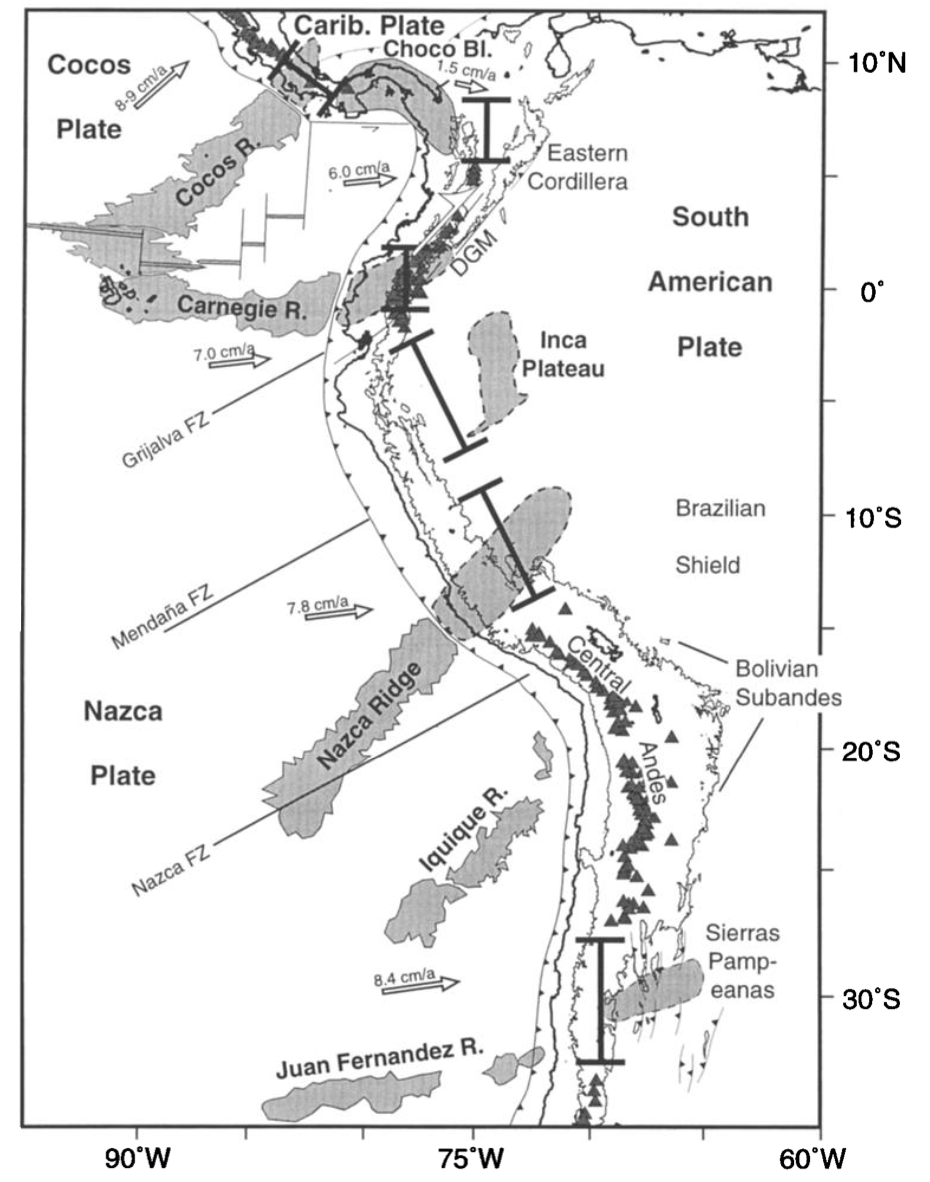
\includegraphics[width=6.5in]{Gutscher_2000_ridge.png}
    \caption{南美洲板塊構造圖,摘自\citealp{Gutscher2000A}。粗黑線標出平坦隱沒段,灰色陰影區標示隱沒的海洋高原與洋脊,三角形為活動火山。板塊聚合速率參考自\citealp{demets1990current}。
    }
    \label{fig::Gutscher_2000_ridge}
\end{figure*}

最早的平坦隱沒模型為\citealp{van2002role}(見圖\ref{fig::van2002}),其利用二維尤拉笛卡爾座標熱化學數值模型成功將增厚的海洋地殼隱沒形成平坦隱沒。為了驗證\citealp{Gutscher2000A}所提出的玄武岩相變延遲,\citealp{van2002role}考慮成分隨時間的變化項,使用額外設定控制玄武岩相變成榴輝岩的延遲時間,為增厚的海洋地殼提供較大的浮力。
然而其研究成果顯示若僅包含增厚的海洋地殼不足以形成平坦隱沒,需要快速聚合速度的存在才能達到平坦隱沒。並且,無論觀測上與實驗上對平坦隱沒的玄武岩相變延遲皆沒有太充足的證明。

\begin{figure*}[ht!]
    \centering
    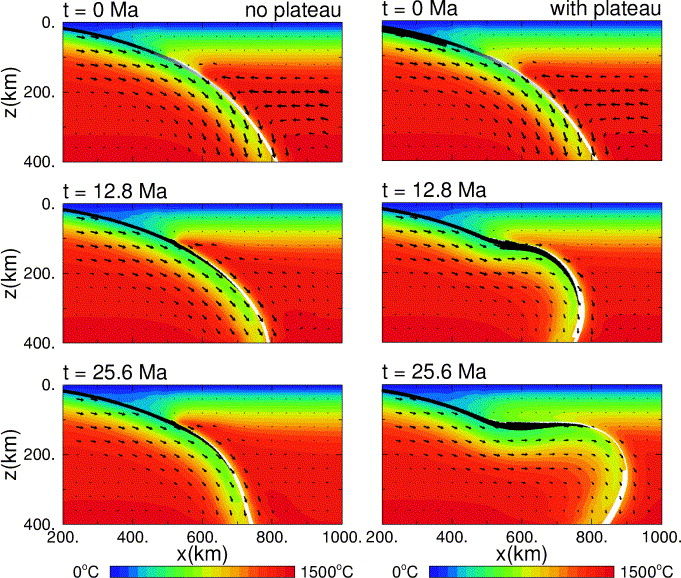
\includegraphics[width=6in]{van2002.png}
    \caption{正常的隱沒帶(左)與包含海洋高原的隱沒帶(右)隨模型時間變化,摘自\citealp{van2002role}。黑白區域繪出海洋地殼的化學成分從玄武岩(黑)到榴輝岩(白)的變化。水平軸為與海溝的距離,背景顏色為溫度。
    }
    \label{fig::van2002}
\end{figure*}

\citealp{Gerya2009}使用二維尤拉笛卡爾座標模型(I2VIS)探討平坦隱沒帶與洋脊隱沒的關係,該模型包含脫水作用、部分熔融與地表高程變化。
為了模擬納茲卡洋脊(Nazca ridge)的存在,模型中隱沒板塊上存在一200公里寬、18公里厚的玄武岩洋脊隱沒進入上覆板塊之下(見圖\ref{fig::Gerya2009})。
模型結果顯示平坦隱沒的形成與洋脊的存在與否無關,只要是密度異常低的海洋岩石圈(見\ref{fig::Gerya2009}(a))皆有利於其形成。
並且,洋脊的存在與岩漿作用是否活躍也無關,當平坦隱沒存在,高溫的地函楔被隱沒板塊閉合,岩漿活動大量減少,有別於在相同情況下沒有平坦隱沒的隱沒帶(見圖\ref{fig::Gerya2009}(b))。
值得一提的是,該模型並沒有考慮玄武岩至榴輝岩的相變過程,平坦隱沒在地殼密度低的情況下發育,系統中的板塊驅動力並不存在。


\begin{figure*}[ht!]
    \centering
    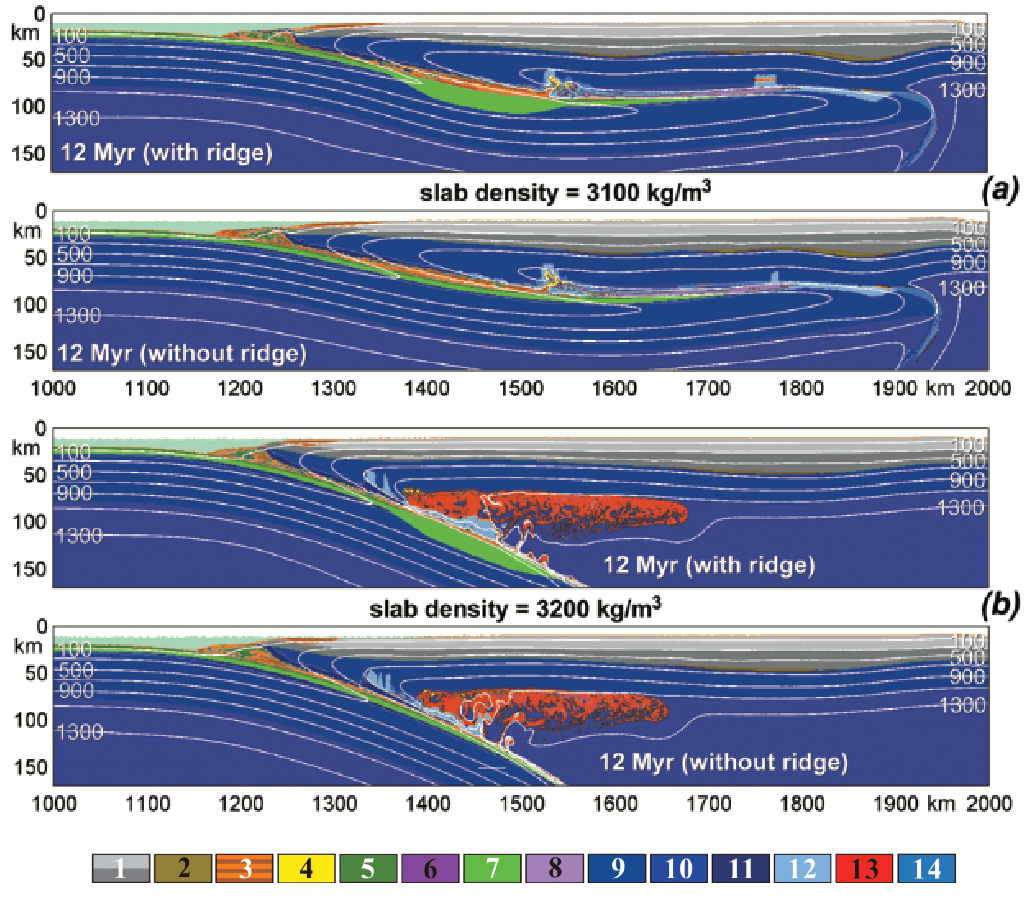
\includegraphics[width=6in]{Gerya_final.pdf}
    \caption{\citealp{Gerya2009}中模型於第12個百萬年的結果。圖組(a)與圖組(b)分別為隱沒海洋地函岩石圈密度$3100 kgm^{-3}$與$3300 kgm^{-3}$的結果。(a)上圖與(b)上圖為包含洋脊隱沒的模型,(a)(b)下圖為不包含洋脊的模型,圖中白線為等溫線。其中,顏色代表不同岩相:1、2=大陸地殼、3、4=沈積物、5、6=玄武岩、7、8=輝長岩、9、10=無水地函、11=蛇紋岩、12、13、14=含水地函。
    }
    \label{fig::Gerya2009}
\end{figure*}

\citealp{Liu2016}利用二維任意拉格朗日-尤拉模型(SOPALE)討論過去拉臘米造山運動(Laramide orogeny)時期($~$80–50 百萬年前)法拉龍板塊(Farallon plate)發生的平坦隱沒事件。
模型的隱沒板塊上設定一段400公里寬的海洋高原,包含18公里厚的增厚玄武岩海洋地殼與36公里厚的斜方輝岩(harzburgite)地函岩石圈。
該模型也假設海洋高原上的玄武岩並不會發生榴輝岩相變,並且斜方輝岩地函岩石圈密度比周遭地函低100 $kg m^-3$。
研究結果表明增厚海洋高原與快速的聚合板塊是平坦隱沒發育的必要條件。
然而由於模型沒有考慮彈性變形,因此並無法很好擬合高程,再者,模型中同樣沒有考慮玄武岩至榴輝岩相變過程。

模型中加入增厚海洋地殼的結果雖然都能讓平坦隱沒發育,但皆存在兩個問題。
第一,上述文獻中所有模型皆是二維模型,這意味著在第三維上有無限延伸的增厚海洋地殼,因此增厚洋殼能在二維假設下提供足夠大的浮力,然而現實中增厚洋殼能造成的浮力效應應遠小於二維模型中的結果。
\citealp{florez2019impact}在三維模型中證明了這一點,他們的研究結果表明若將現在自然界中最大的洋脊隱沒進入地函中,其所提供的浮力也只會造成海洋板塊傾角減少原先的10度。
第二,過去研究針對玄武岩至榴輝岩相變過程並沒有完善的解釋,\citealp{van2002role}所使用的相變延遲現象無法用實驗所證明,而剩餘研究皆沒有考慮此相變過程,與自然界的觀測無法吻合。

若從自然界中來看,確實有許多區域皆有海脊隱沒的證據,例如勘察加半島(Kamchatka)有皇帝海脊(Emperor Ridge)隱沒、琉球(Ryukyu)有大東海脊(Daito Ridge)隱沒以及馬里亞納(Mariana)與馬庫斯—內克海脊(Marcus-Necker Ridge)隱沒,然而只有秘魯與智利有平坦隱沒的特徵。
此外,在墨西哥有平坦隱沒的特徵,然而墨西哥沒有任何海脊或海洋高原的隱沒紀錄,因此增厚的海洋地殼發生平坦隱沒的理論近年來逐漸站不住腳(\citealp{schellart2020control}; \citealp{Schellart2021})。

\subsection{實現數值模型中增加的地函動水壓力矩}
\citealp{tovish1978mantle}計算隱沒帶中的角流(corner flow)指出非牛頓流體的地函可以產生極大的地函流吸力(mantle flow suction force),導致動水壓力矩(hydrodynamic pressure torque)足夠抵抗重力力矩,形成平坦隱沒。
\citealp{Manea2007}使用二維模型CitcomS研究隱沒帶中脫水作用、地函黏滯度與動水壓力對隱沒板塊幾何的影響。
模型的地函楔中假設隱沒板塊脫水作用會產生一梯型低黏滯度區,詳見圖\ref{fig::Manea2007}。較低的黏滯度增加地函楔中的壓力,導致板塊兩側的壓力差減少,大幅度減少隱沒系統的地函流吸力。
先前研究計算隱沒板塊力矩解析解時並沒有考慮隱沒帶中的脫水作用影響,因此高估地函吸力的量值。
數值模型雖然可以透過測試地函黏滯度量值獲得平坦隱沒模型,然而黏滯度量值大範圍的不確定同時也是模型硬傷,多個數量級的黏滯度難以利用時驗證明模型的真實性。

\begin{figure*}[ht!]
    \centering
    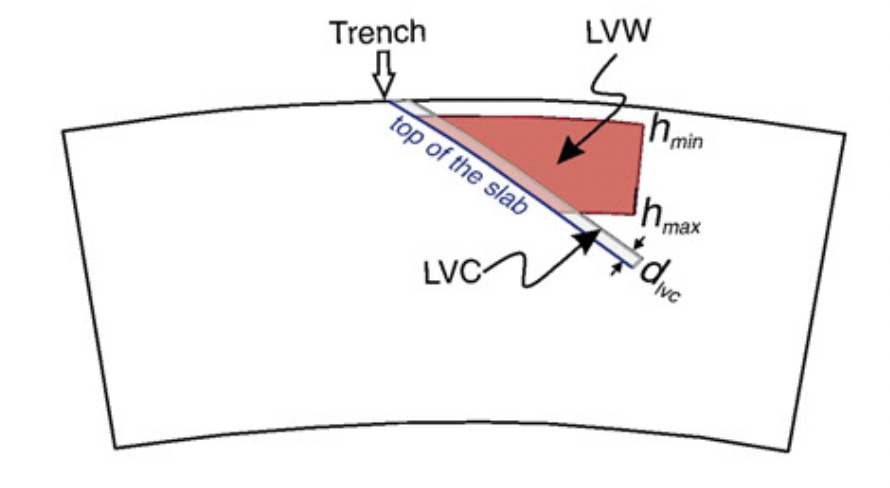
\includegraphics[width=3in]{Manea2007.png}
    \caption[\citealp{Manea2007}模型中所設定的低黏滯度與低黏滯度通道區域,摘自\citealp{Manea2007}]{\citealp{Manea2007}模型中所設定的低黏滯度與低黏滯度通道區域,摘自\citealp{Manea2007}}
    \label{}
\end{figure*}

\citealp{Thermal2012}利用包含牛頓流體(diffusion creep)與非牛頓流體(dislocation creep)的複合流變學不可壓縮流二維模型,討論上覆板塊的溫度構造與平坦隱沒的關係,模型中海溝位置不隨時間改變。
他們的結果認為冷硬的大陸岩石圈可以促使隱沒板塊角度變低,同時他們也計算了模型中重力力矩與吸力力矩的大小。
他們的結論支持平坦隱沒不是一個穩態(steady-state)狀態,並且只有在隱沒剛開始發生的時間點才會出現。
不過這便違反了現生平坦隱沒的特色,無論是智利、秘魯或墨西哥的平坦隱沒都不是隱沒初期的構造,三個地區的隱沒帶已經持續超過200個百萬年,皆是近期(<15 個百萬年)才有平坦隱沒事件發生。
另外,該模型使用的溫度構造皆是平板模型(plate model),嚴格上不適用於大陸岩石圈。

\citealp{Manea2012Chile}利用三維模型模擬過去30個百萬年來智利區域的隱沒帶動態行為,邊界條件與\citealp{Thermal2012}幾乎相同。模型開始先是普通的隱沒帶模型,在隱沒帶發育成熟後,額外施加一段邊界條件強迫智利海溝後撤,發現海溝後撤能夠施加給隱沒板塊的地幔流吸力(suction),不過該吸力量值不足以讓巨大厚重的海洋板塊變平坦。
\begin{figure*}[ht!]
    \centering
    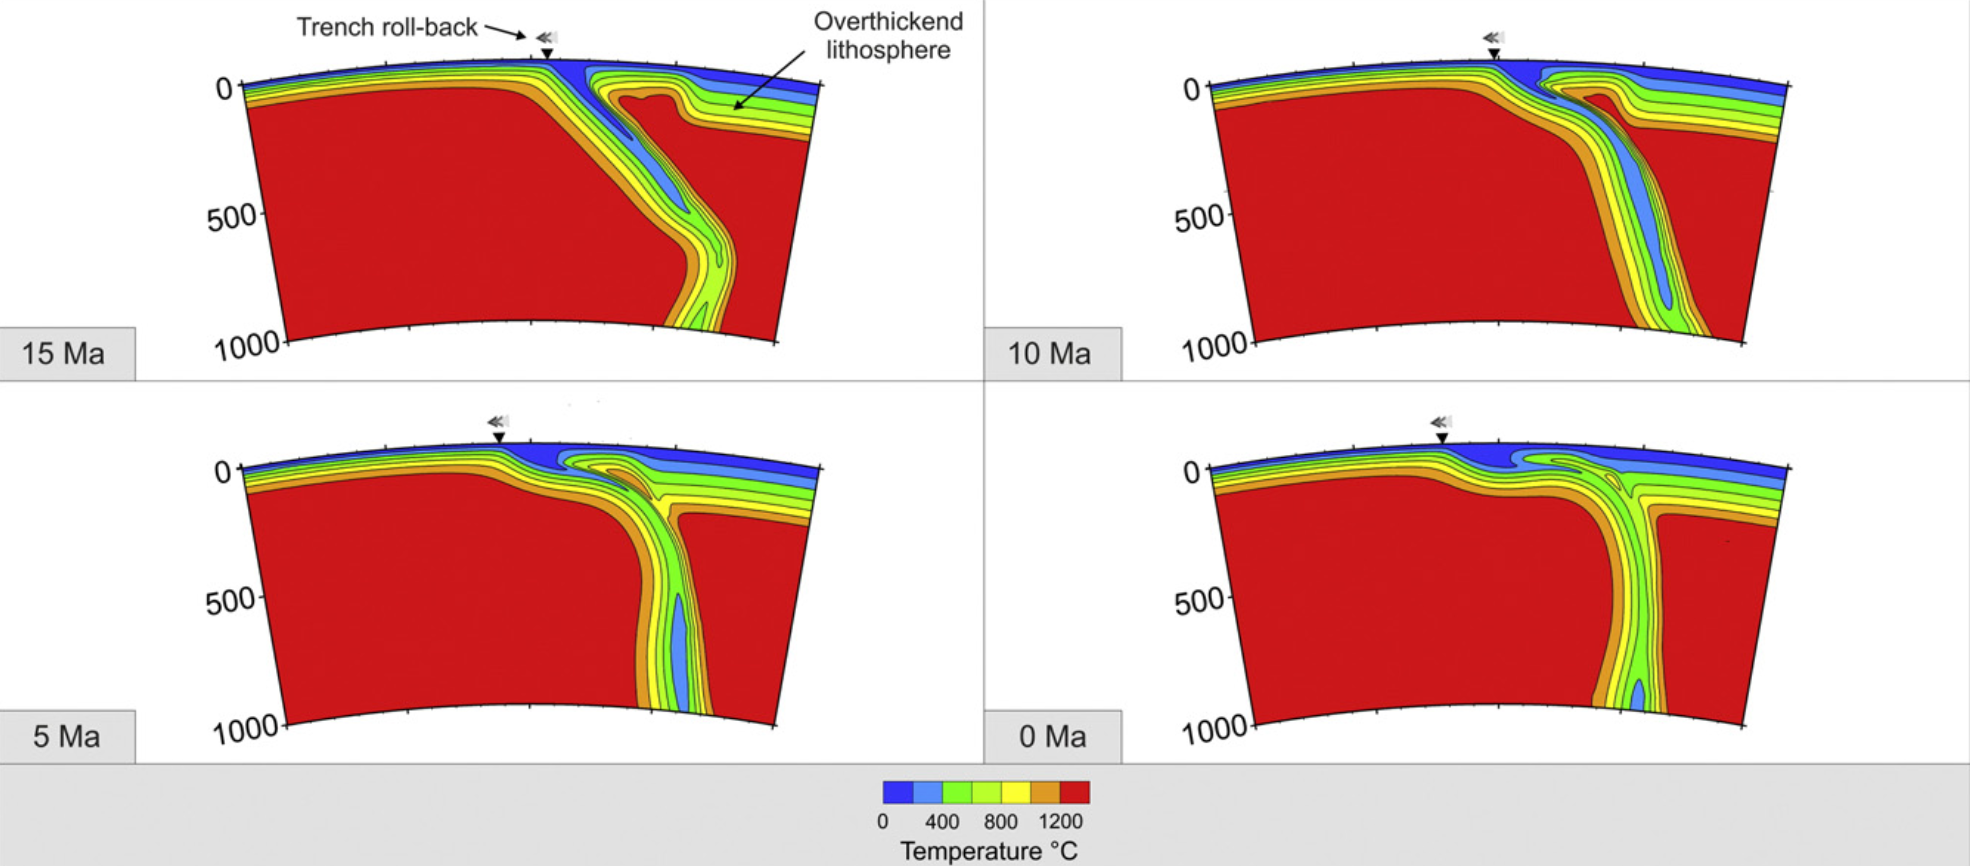
\includegraphics[width=6in]{Manea 2012.png}
    \caption{\citealp{Manea2012Chile}中的智利平坦隱沒模型,模型中同時加入海溝後撤與增厚大陸岩石圈可以讓平坦隱沒發育。
    }
    \label{fig::Manea 2012}
\end{figure*}
由於地震學研究表明南美洲大陸包含數個古老克拉通(craton)地塊,\citealp{Manea2012Chile}便將模型中上覆板塊厚度增厚,代表冷硬的克拉通構造,該地質設計讓隱沒帶下方地函流的動力壓力增加(見圖\ref{fig::Manea 2012})。
因此他們得出的結論是需要同時有海溝後撤與克拉通的存在才會觸發平坦隱沒,這是首次在不更改隱沒板塊狀態、僅利用增加動水壓力產生的平坦隱沒模型。
他們的模型中沒有考慮地殼與地函的密度差,也沒有考慮任何相變過程。
隨後\citealp{Liu2016}效仿同樣的機制,將過去普遍認為存在於北美板塊西部下方的科羅拉多高原山根放入模型中,模擬法拉龍板塊平坦隱沒演化。
然而他們的研究表示克拉通與山根的存在只是加快平坦隱沒的形成,但真正觸發平坦隱沒的機制是增厚且沒有榴灰岩相變的海洋地殼,亦即動水壓力矩對隱沒帶的影響並不大。


\citealp{Hu2016}重複與\citealp{Manea2012Chile}同樣的實驗,使用三維模型CitcomS模擬整個南美洲海溝45個百萬年以來隱沒帶的演化。
這次他們將觀測資料當作模型邊界條件,逐一分析海溝後撤、海洋高原隱沒與克拉通山根的存在對模型的影響。
在加入克拉通的模型中,隱沒板塊傾角有降低的趨勢,不過並不足以形成平坦隱沒,僅能視為低傾角隱沒。
隨後模型加入隱沒的海洋高原,隱沒傾角在地區上顯著降低,表明隱沒的海洋高原才是平坦隱沒發育的主因。
然而該模型並沒有考慮隱沒帶脫水作用與玄武岩相變的影響。
固動水壓力矩與重力力矩對平坦隱沒發育的角色仍然存在分歧。

\section{研究動機}
最簡單直接的平坦隱沒概念模型可以透過改變隱沒系統的重力力矩達成,尤其是早期的隱沒洋脊理論。然而過去研究針對玄武岩至榴輝岩相變過程並沒有完善的物理機制解釋。
相較於隱沒帶重力力矩的直觀性,動水壓力矩增大的條件與其對隱沒帶造成的影響較難以用單一的地質構造或特性約束。
\citealp{Manea2017}與\citealp{Yan2020}提及隱沒帶脫水作用應是對動水壓力力矩有重大影響的因素之一。
此外,上述研究皆是以南美洲秘魯與智利的平坦隱沒當作模型藍本,少部分考量法拉龍板塊的平坦隱沒事件,墨西哥區域尚未有平坦隱沒的數值模型被提出。
在墨西哥,隱沒板塊上沒有任何隱沒海脊的紀錄,上覆板塊也沒有任何克拉通存在的證據,因此墨西哥的平坦隱沒可能具有不為人知的機制存在。
本研究將著重在探討動水壓力力矩在哪些環境下會發生改變,並且在考慮玄武岩至榴輝岩相變的過程下模擬平坦隱沒的發育,此外,本研究期待能利用數值模擬得到墨西哥平坦隱沒模型,填補過去尚未成熟的平坦隱沒機制。
接下來會先針對各個平坦隱沒區域的觀測資料進行文獻回顧,包含納茲卡隱沒帶的秘魯、智利平坦隱沒區域以及科科斯隱沒帶上的墨西哥平坦隱沒。

\section{Geophysical observations in Cocos subduction zone}
相較於南美洲,墨西哥的平坦隱沒較晚才被發現。墨西哥平坦隱沒區域位在.....,該地區的地震活動度較低,並且地震事件集中在距海溝100公里以內的範圍,因此過去難以描繪出科科斯板塊隱沒帶的幾何形狀。

\citealp{pardo1995}藉由當地地震目錄重新定位震源判斷在墨西哥中部的板塊交界處下方有平坦隱沒存在,為最早對墨西哥區域的平坦隱沒研究。
\citealp{PerezCampos2008}使用接收函數方法(receiver function method)得到清晰的平坦隱沒板塊特徵,如圖\ref{fig::receiverfunction2008}。
該剖面北部顯示大陸地殼與地函之間的莫合面(Moho),見\ref{fig::receiverfunction2008}上圖的接收函數影像;南部則些微顯示一個水平介面,如圖\ref{fig::receiverfunction2008}左下,深度落在40-50公里之間,平坦段長度約100公里。
有別於南美洲區域的平坦隱沒,墨西哥的平坦隱沒深度幾乎與地殼貼齊,他們認為具有長達100公里的板塊交界面可能還保留脆性變形的流變特徵,理論上應有強耦合特性,亦即該地區應該容易累積大量應力產生多起地震事件。然而正如前面所提到,墨西哥平坦隱沒段的地震活動度極低,甚至在格雷羅州擁有世界知名的格雷羅無震帶(Guerrero gap),與平坦隱沒的存在產生矛盾。GPS研究也支持該地區並不是強耦合板塊介面。並且,墨西哥區域的平坦隱沒持續時間($~$15 Ma)比安地斯山脈平坦隱沒來得長($~$4-5 Ma),然而墨西哥平坦隱沒上方並沒有顯著的水平壓縮現象(\citealp{nieto2006latest}; \citealp{moran2007cenozoic})。
對此,板塊交界處需要有可行機制解釋該地區弱耦合現象。

\begin{figure*}[ht!]
    \centering
    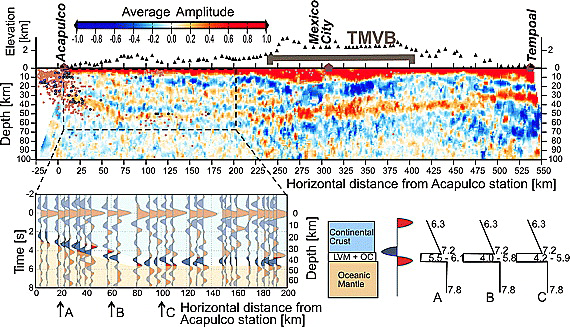
\includegraphics[width=6in]{2008receiverfunction.png}
    \caption[墨西哥平坦隱沒區域接收函數結果,摘自\citealp{PerezCampos2008}]。{上圖:黑色三角形表示測站沿剖面的位置,高程被放大10倍。粗棕色線表示跨墨西哥火山帶(TMVB, Trans-Mexican Volcanic Belt)的範圍。上圖接收函數影像中標出沿剖面50公里範圍內的震源(粉紅色點來自SSN地震目錄;綠色點來自\citealp{pardo1995}重新定位結果)位置。下方左圖:顯示沿平坦隱沒板塊的一次遠震事件的接收函數。下方中間圖:說明了相應的模型(LVM(low velocity mantle) = 低速地函和 OC(oceanic crust) = 海洋地殼)。下方右圖:根據左下圖接收函數模型中A、B和C位置上的P波速度模型。
    }
    \label{fig::receiverfunction2008}
\end{figure*}

\citealp{PerezCampos2008}在平坦隱沒板塊段與大陸板塊交界處中,初步判斷有一約略10±3公里厚的低速帶,速度模型如圖\ref{fig::receiverfunction2008}右下。
該低速層很可能是弱耦合現象的主因。
\citealp{Song2009}利用平坦隱沒上方地區性慢速滑移事件的轉換SP波進行波形模擬,確認該低速層厚度約3-5公里,並且其$V_s$速度約每秒2.0-2.7公里。
爾後\citealp{Song2012SC}發現該低速區的地震非均向性傾角方向與隱沒板塊介面傾角方向有20 ± 10$^{\circ}$的夾角,與S(葉理面)-C(剪切面)糜棱岩中發育的晶體方向一致,再藉由該低速區的訊號特徵,包含強烈的地震非均向性(>5$\%$)、高Vp/Vs比值、高反射率(high seismic reflextivity)與Vs顯著降低(-15-20$\%$),判斷該低速層應是擁有大體積黏土礦物(例如:滑石)的變質岩,並且同時存在高孔隙流體(\citealp{Kim2012})。

\begin{figure*}[ht!]
    \centering
    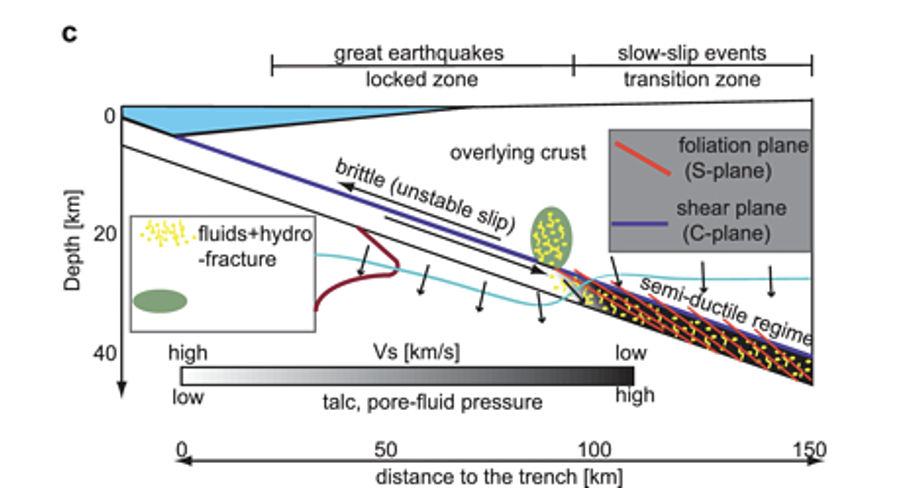
\includegraphics[width=6in]{SCanisotropy.png}
    \caption{墨西哥隱沒帶板塊介面附近剪切帶結構示意圖(\citealp{Song2012SC}
    )。大地震主要發生在鎖定區(locked zone)和脆性(brittle)變形區域。慢速滑移事件(slow-slip event)主要發生在過渡帶(transition zone)和半韌性區域(seni-ductile regime),Vs非常低,且非均向性極強。岩石流變轉換由350$^{\circ}$等溫線(淺藍色線)分開,導致應力梯度形成且方向與黏土礦物中流體壓力相反,導致低速帶的形成。這些低速帶流體導致板塊介面處於低耦合狀態,並且主導該地區慢速滑移事件的生成。
    }
    \label{fig::SCanisotorpy2012}
\end{figure*}

\begin{figure*}[ht!]
    \centering
    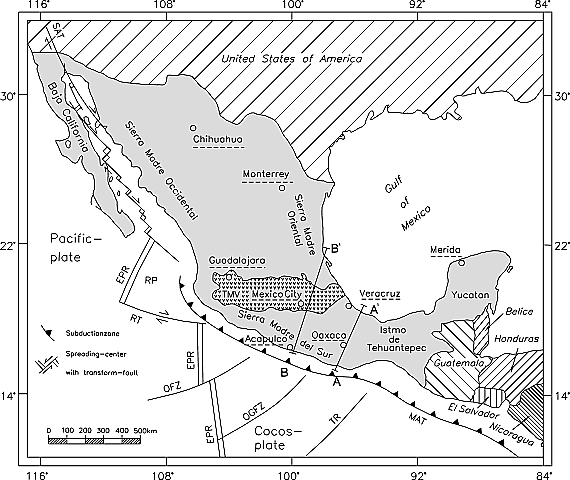
\includegraphics[width=3in]{MT_line.png}
    \caption{\citealp{MT2006}中所使用的大地電磁剖面位置圖,本研究僅使用BB'剖面。
    }
    \label{fig::MT_site}
\end{figure*}

\begin{figure*}[ht!]
    \centering
    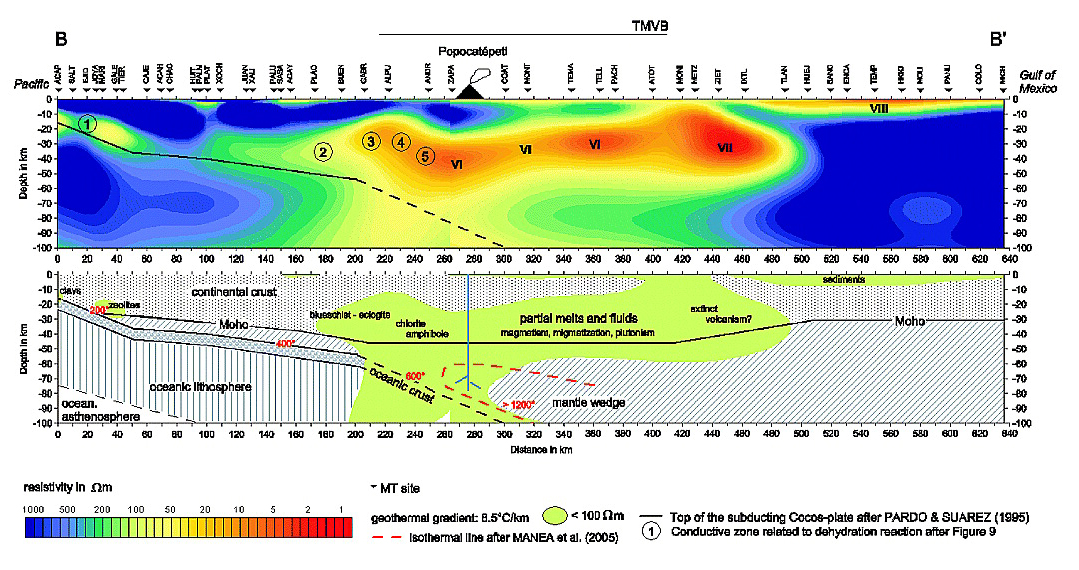
\includegraphics[width=6in]{MT_profile.png}
    \caption{墨西哥平坦隱沒區域的導電率異常剖面圖與解釋圖,摘自\citealp{MT2006}。上圖為電阻率異常結果剖面,所繪之隱沒板塊位置參考自\citealp{pardo1995}結果,最上方標示跨墨西哥火山帶的範圍。圖中每個數字圈皆代表隱沒帶上岩石發生向變後脫水的位置。下圖為電阻異常解釋圖,綠色區域為電阻異常低區(<100 $\Omega m$)。在平坦隱沒段結束處有多個岩石相變事件發生,隱沒板塊上出現大範圍導體。
    }
    \label{fig::MT_profile}
\end{figure*}

\citealp{MT2006}利用大地電磁法獲得墨西哥平坦隱沒區域的導電率異常剖面(見圖\ref{fig::MT_site}),發現在平坦隱沒結束前、隱沒板塊上方存在高導體區域,可能是隱沒板塊上物質因大量脫水產生。
該圖\ref{fig::MT_site}中編號2-5的弧前高導體區域與慢速滑移事件位置相吻合,增加了編號2-5導體物並非岩漿庫,而是流體存在的證據。
大量流體存在意味著脫水作用活躍,在隱沒板塊進入較高溫高壓環境下,釋放出的水分進入地函鍥中,導致蛇紋岩化橄欖岩的生成。
對此,\citealp{Manea2013}認為低速層可能不完全是地殼物質,而是過去殘留下的地函蛇紋岩成份,然而其內容物目前尚未完全了解。

\section{Geophysical observations in Nazca subduction zone}

\section{Magmatism observation in flat slab subduction}

\section{End}
第一章首先介紹地球動力學研究目的與平坦隱沒區域(包含墨西哥與南美洲)的地球物理觀測資料語言將資料結果,並說明本研究的動機與目的。第二章說明數值模擬的研究原理。第三章呈現研究結果,並且在第四章更進一步討論分析。最後於第五章歸納出本研究重要結論。